\section{Recurrent Neural Networks (RNNs)}

\begin{frame}\frametitle{\subsecname}

\begin{itemize}
\item Feedforward netwroks:\\

\underline{Data}:
\begin{equation*}
\Big\{ \left(\vec x^{(\alpha)}, \vec y^{(\alpha)}_{\mathrm{True}} \right) \Big\}\,,\quad \alpha = 1,\ldots,p
\end{equation*}

\pause

\begin{itemize}
\item any two sample pairs $\left(\vec x^{(\alpha)}, \vec y^{(\alpha)}_{\mathrm{True}} \right)$ and $\left(\vec x^{(\alpha')}, \vec y^{(\alpha')}_{\mathrm{True}} \right)$ are assumed to be \iid
\item Their respective predictions $\vec y(\vec x^{(\alpha)}; \vec w)$ and $\vec y(\vec x^{(\alpha')}; \vec w)$ are also independent from one another.
\end{itemize}

\pause

\item RNN \corresponds~Neural network with loops.\\

\underline{Data}:\\

\begin{equation*}
\Big\{ \left(\vec x^{(\alpha,t)}, \vec y^{(\alpha,t)}_{\mathrm{True}} \right)_{t=1}^{n_{\alpha}} \Big\}\,,\quad \alpha = 1,\ldots,p
\end{equation*}

\pause

\begin{itemize}
\item $p$ \iid sequences
\item each sequence $\alpha$ contains $n_{\alpha}$ time steps
\item Use information from the previous step to predict the next step.
\end{itemize}

\end{itemize}

\end{frame}


\subsection{Basic RNN}


\begin{frame}\frametitle{\subsecname}

\begin{figure}[ht]
     \centering
	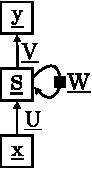
\includegraphics[width=0.2\textwidth]{img/rnn}
     \mode<article>{
	\caption{Basic RNN architecture}
	}
	\label{fig:rnn} 
\end{figure}
\end{frame}

\begin{frame}\frametitle{\subsecname}

Omitting sequence index $\alpha$
\begin{figure}[ht]
     \centering
	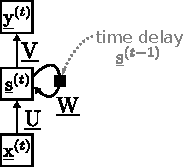
\includegraphics[width=0.2\textwidth]{img/rnn_time_delay}
     \mode<article>{
	\caption{Basic RNN architecture}
	}
	\label{fig:rnn} 
\end{figure}

We measure the activities of the neurons in the RNN:



\end{frame}

\begin{frame}\frametitle{\subsecname}

\begin{figure}[ht]
     \centering
	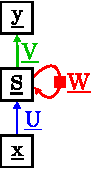
\includegraphics[width=0.2\textwidth]{img/rnn_colored}
     \mode<article>{
	\caption{Basic RNN architecture}
	}
	\label{fig:rnn} 
\end{figure}

Let
\begin{itemize}
\item[] $N$ be the number of input variables $\rightarrow$ $\vec x^{(t)} \in \R^N$
\item[] $H$ be the number of hidden nodes
\item[] $M$ be the number of output nodes
\end{itemize}

Identify the free parameters (trainable weights) of the network:

\begin{itemize}
\item input-to-hidden: ${\color{blue} \vec U = (\vec u_1,\ldots, \vec u_i, \ldots,\vec u_H)} \in \R^{H,N}$
\item hidden-to-hidden: ${\color{red} \vec W = (\vec w_1,\ldots, \vec w_j, \ldots,\vec u_H)} \in \R^{H,H}$
\item hidden-to-output: ${\color{green} \vec V = (\vec v_1,\ldots, \vec u_j, \ldots,\vec u_H)} \in \R^{H,H}$
\end{itemize}


We measure the activities of the neurons in the RNN:

Omitting sequence index $\alpha$




\end{frame}
